\documentclass[]{article}

\usepackage{graphicx}

%opening
\title{3D-printable micropipette (Figures and Tables)}
\author{}

\begin{document}

\maketitle

\begin{figure}
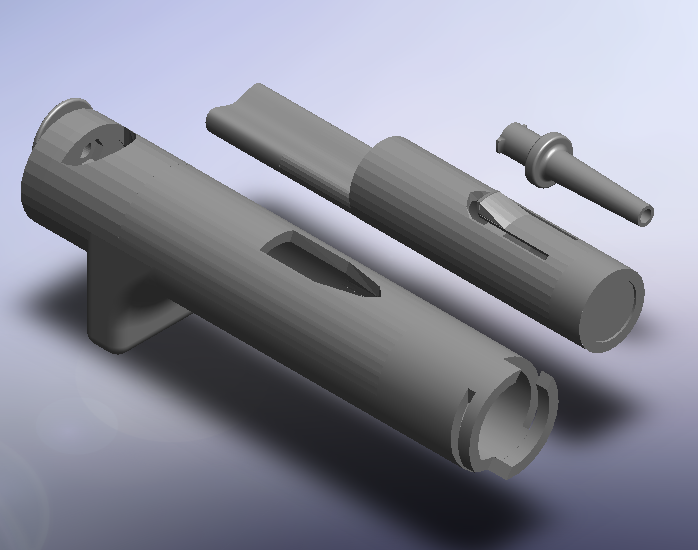
\includegraphics[scale=0.4]{fig1.PNG}
\caption{
{\bf CAD rendering of printable parts.}  Three parts are printed: the body, plunger shaft, and luer-lock adapter for pipette tips.
}
\label{figure1}
\end{figure}

\begin{figure}
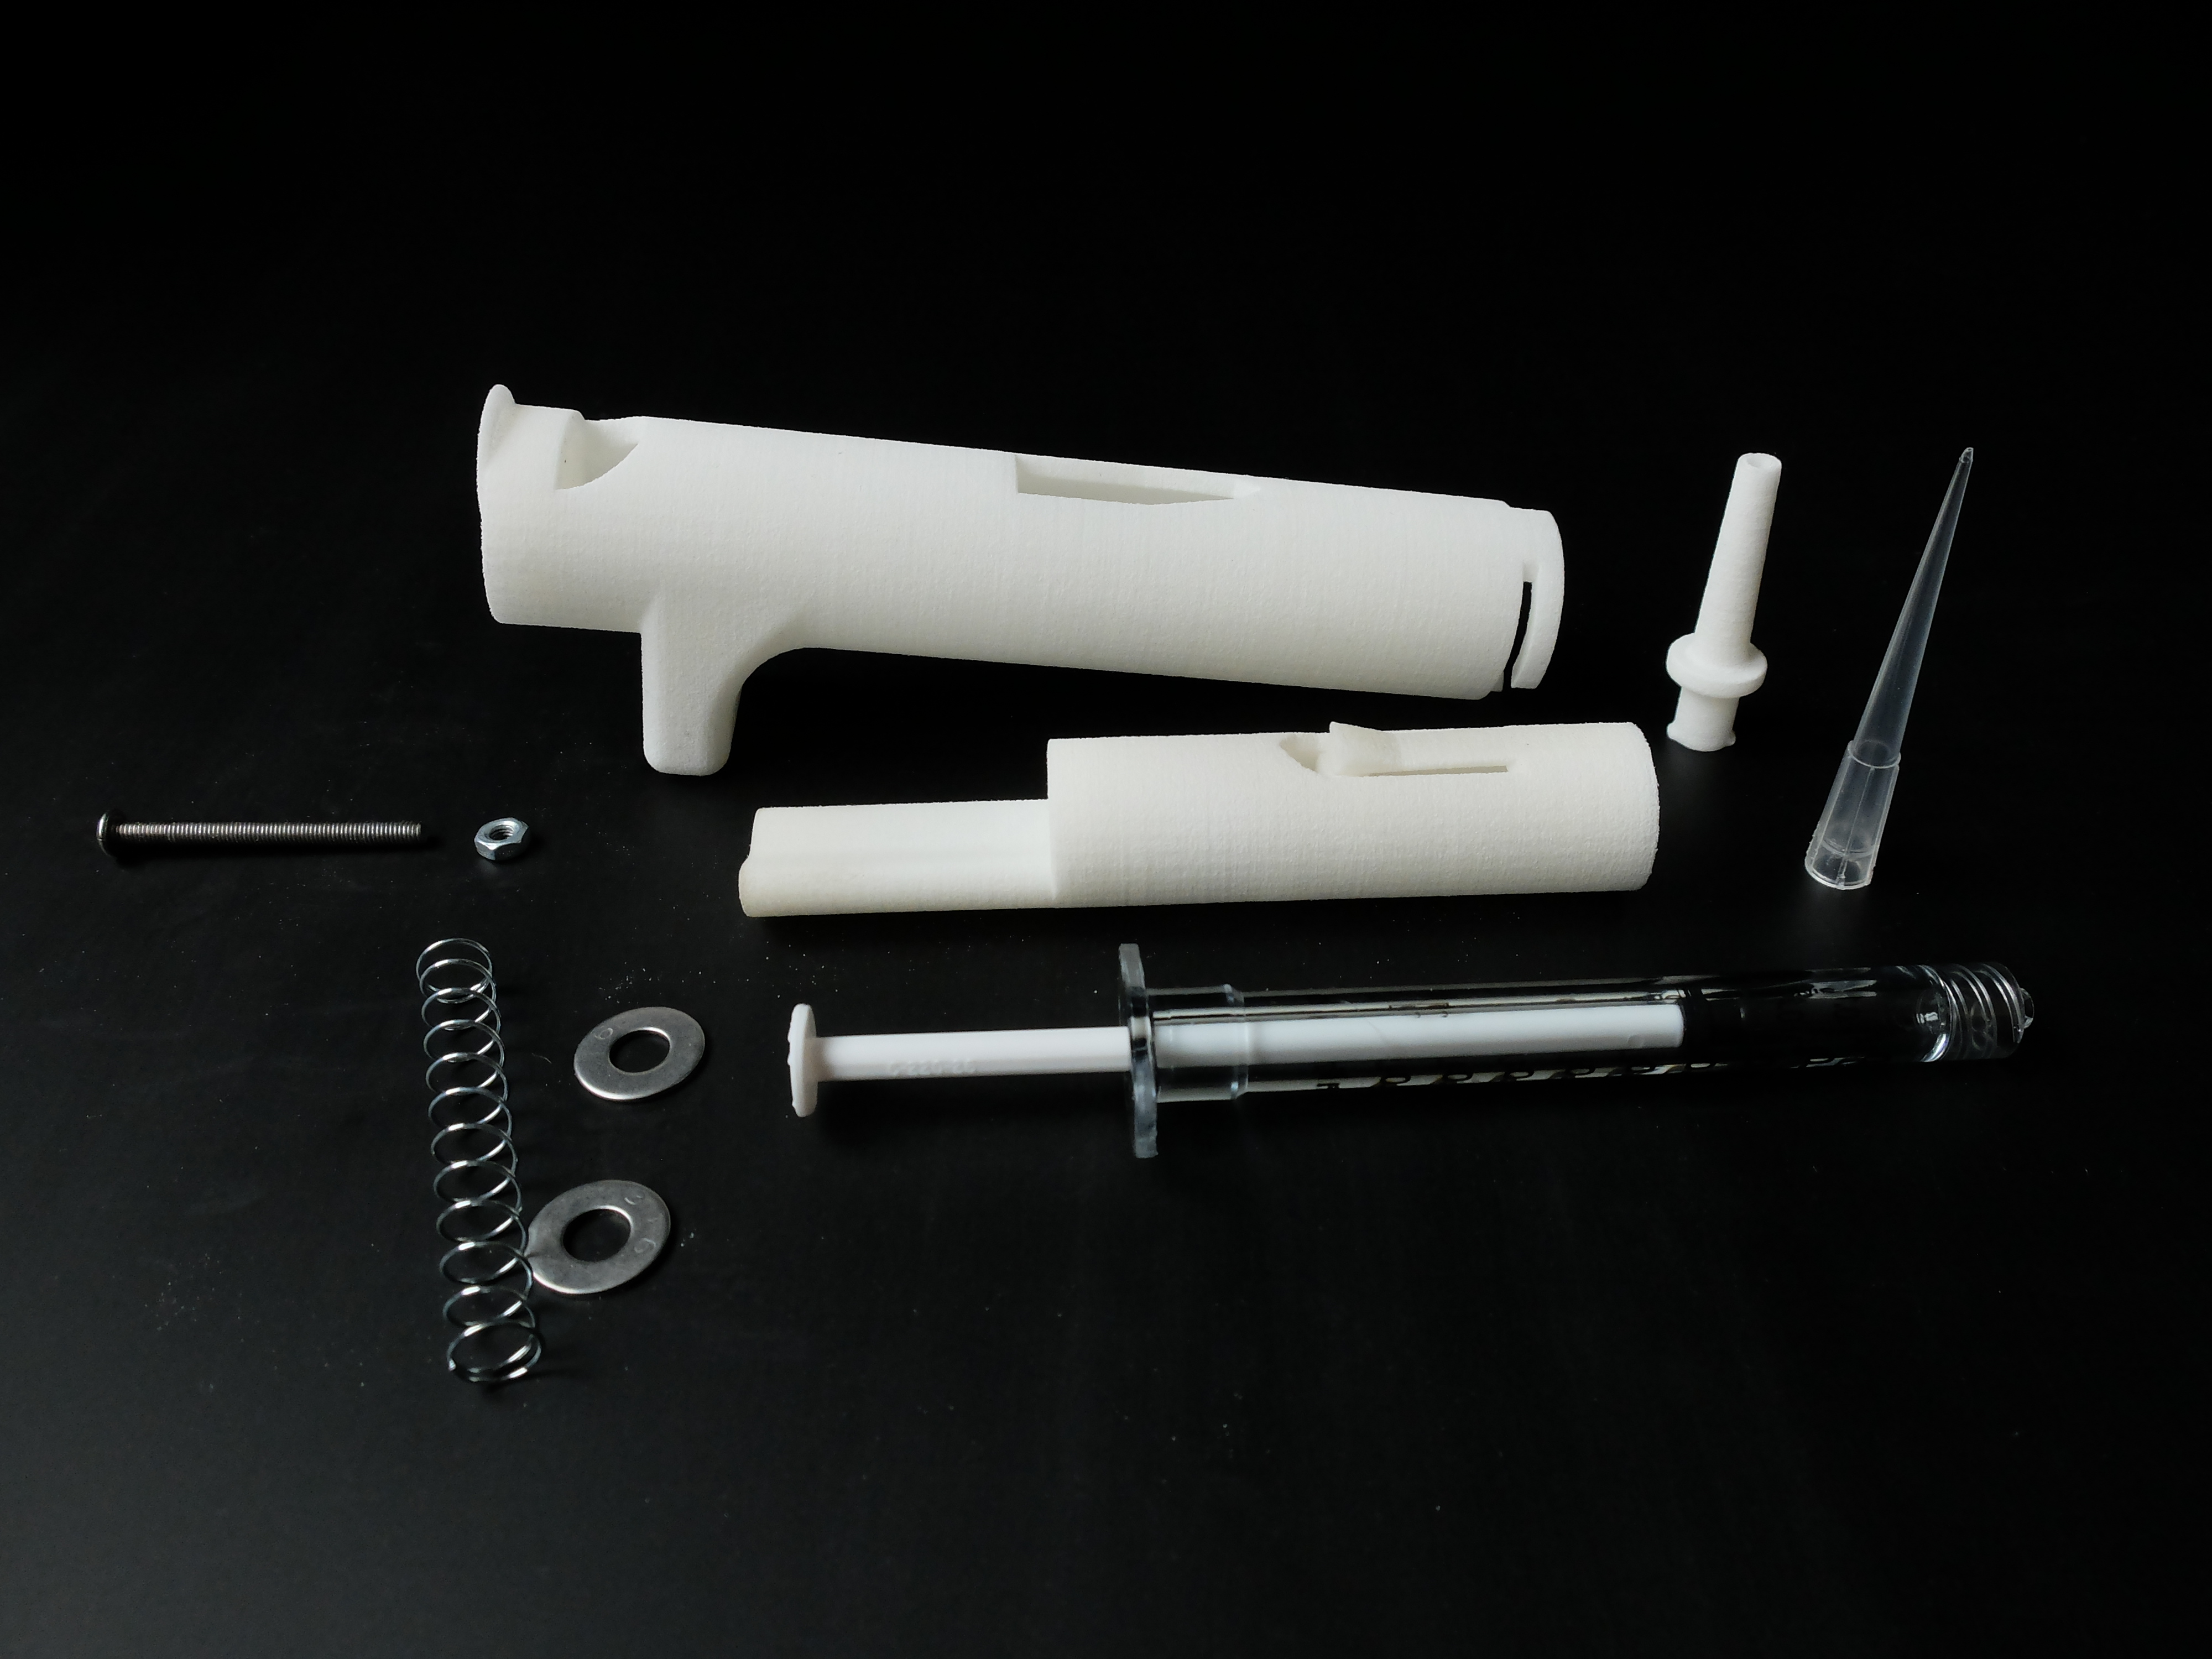
\includegraphics[scale=0.04]{pipette-disassembled.JPG} % take image out for final manuscript
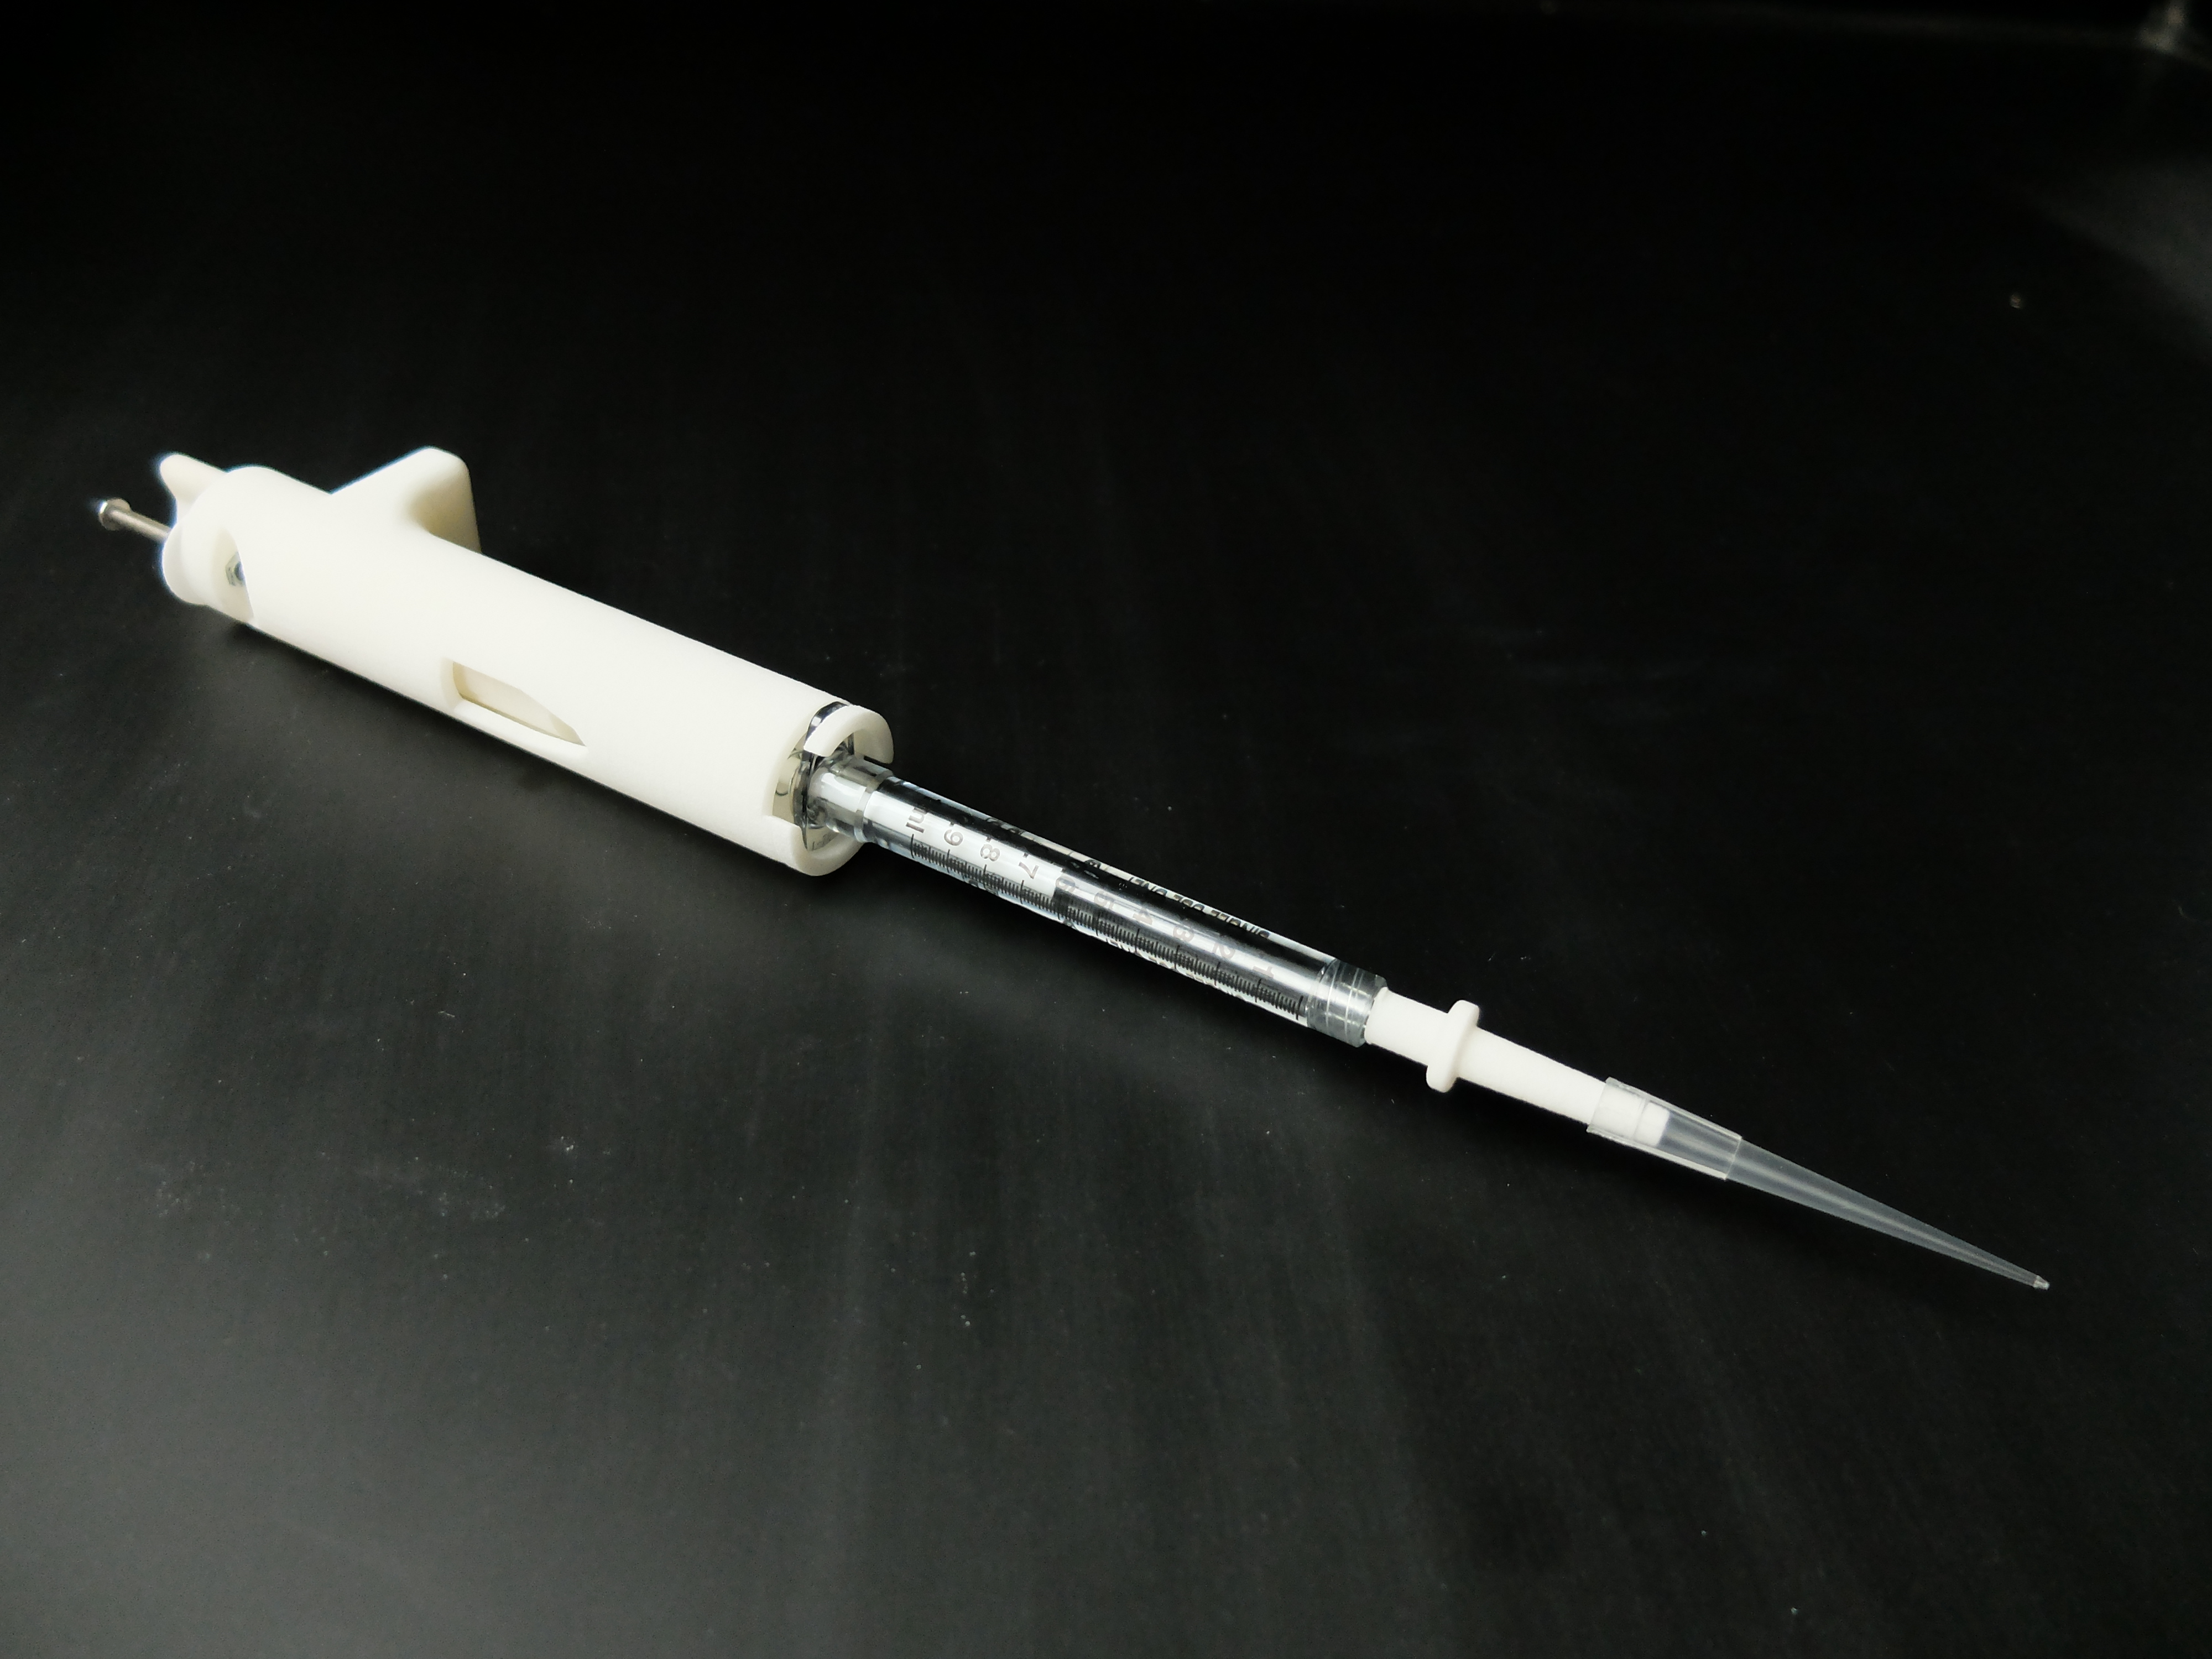
\includegraphics[scale=0.04]{pipette-assembled.JPG} % take image out for final manuscript
\caption{
{\bf Photos of pipette.}  The pipette is composed of three printed parts, a 1 mL syringe and some additional hardware.  
}
\label{figure2}
\end{figure}

\begin{table}[!ht]
\caption{
\bf{Comparison of Accuracy and Precision}}
\begin{tabular}{|c|c|c|c|}
\hline
    Target Volume & 20 $\mu$L & 50 $\mu$L & 200 $\mu$L  \\
    \hline
    Printed Pipette & 196.4 $\pm$ 2.2 & 53.5 $\pm$ 1.8 & 19.5 $\pm$ 0.6 \\
    Commercial Pipette & 204.5 $\pm$ 2.9 & 49.9 $\pm$ 0.1 & 19.9 $\pm$ 0.2 \\
    \hline
\end{tabular}
\begin{flushleft} Average measured volume by weight and standard deviation.
\end{flushleft}
\label{tab:comp}
 \end{table}

\begin{figure}
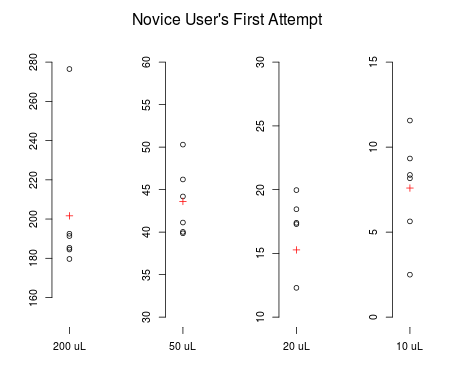
\includegraphics[scale=0.7]{fig3.png}
\caption{
{\bf Novice user's first attempt.} Measurments of novice user's first attempt at adjusting the pipette to target volumes.
}
\label{figure3}
\end{figure}


%\begin{abstract}

%\end{abstract}

%\section{}

\end{document}
